
\documentclass[11pt]{report}

\usepackage{longtable}

\usepackage{epsfig}

\usepackage{USCthesis2004}

% Yu-Fen's changes to the defaults
  % Titles of sections:
  %       \renewcommand{\refname}{fREFERENCES}
          \renewcommand{\bibname}{BIBLIOGRAPHY}
  % Fonts for these titles
        \renewcommand\contentsname{\centerline{\bf Table of Contents}}
        \renewcommand\listfigurename{\centerline{\bf List of Figures}}
        \renewcommand\listtablename{\centerline{\bf List of Tables}}


%new environments

\newtheorem{definition}{Definition}

\newtheorem{theorem}{Theorem}

\newtheorem{proposition}[theorem]{Proposition}

\newtheorem{lemma}[theorem]{Lemma}

\newtheorem{corollary}[theorem]{Corollary}

\newtheorem{remark}{Remark}



% roman numbering

% remove the next two lines for arabic numbering

\renewcommand{\thechapter}{\Roman{chapter}}

\renewcommand{\theenumi}{(\roman{enumi})}



\title{Roslyn: The Tour Guide Robot}



\author{Jared Rhizor, Timothy Sweet, and Nishok Yadav}



\date{May 2014}



% You don't need the next line if the copyright year is the current year

\renewcommand{\copyrightyear}{2014}


% You can adjust the line spacing by redefining \stretchratio.

% For example  \renewcommand{\stretchratio}{1}

% will typeset the document in single spacing.
\renewcommand{\stretchratio}{2}



\ProcessOptions
\begin{document}



\maketitle



\begin{preface}



\pagebreak   % Dediciation


\pagebreak   % Acknowledgements

\mbox{}



\vspace{0.5in}

\begin{center}

{\Large \bf Acknowledgements}

\end{center}

The authors would like to thank of number of people who made this project possible. First, our advisor, Dr. Dave Feil-Seifer, whose enthusiasm and support drove this project to success. Second, the University of Nevada Robotics Research Lab, including its directors Dr. Dave Feil-Seifer (again) and Dr. Monica Nicolescu for providing us a place to work and equipment to use. Third, to Dr. Sergiu Dascalu for providing guidance on the project as a whole, and especially in developing all of the specifications, diagrams, etc. in this document. Fourth, to the University of Nevada, Reno Honors Program and Office for Interdisciplinary and Undergraduate Research for providing funding for Roslyn’s additional hardware. Fifth, to Team 4 (Luke, Jessie, Jake, and Blake) from our 2014 CS 426 Senior Projects course, who helped at every step of development, contributing their time, expertise, food, and study partners. Sixth, to the Open Source Robotics Foundation, Willow Garage, and the entire Robot Operating System community for doing most of the heavy lifting in developing the robotic control and interface components.

%Uncomment next line if you want to add acknowledgements to content

%\addcontentsline{toc}{chapter}{Acknowledgements}





\begin{singlespace}

 \tableofcontents   % content

 \listoffigures     % list of figures

\end{singlespace}



\pagebreak

\begin{abstract}

The tour guide robot Roslyn is an autonomous system that can provide tours to anybody on the second floor of the Scrugham Engineering and Mines building. The robot is not only able to navigate the halls, but navigate them in a socially acceptable manner. This means it does not collide with pedestrians while in motion and takes walking speed into consideration. In order to interact with the user, there is a touch-screen display mounted on top of the moving robot base. As the robot moves throughout the hall, information appears on the screen related to the landmarks being passed (i.e. laboratories and offices). The user is also able to select a destination on the screen in order to begin the tour.

\end{abstract}

\addcontentsline{toc}{chapter}{Abstract}



\end{preface}


\chapter{First Chapter}

The tour guide robot Roslyn is a socially aware autonomous system that can lead tours of the Computer Science and Engineering Department at the University of Nevada, Reno. This requires socially acceptable navigation within the second floor of the Scrugham Engineering and Mines building.
Tours of the Computer Science and Engineering Department are currently given by faculty and staff, or student ambassadors (typically from other departments). This creates some difficulties for visitors:
\begin{itemize}
 \item A tour can only be scheduled when a faculty or staff member is available. This may conflict with class times, office hours, or other responsibilities
 \item Giving tours distracts faculty and staff from their normal studies, teaching, research, etc. especially with large groups
 \item Tours given by student ambassadors are generally limited to superficial knowledge of the department, such as the location of the department office. A typical student ambassador would not be able to answer specific questions about a program, lab, or other facility. 
\end{itemize}

A robotic tour guide could address many of these issues:
\begin{itemize}
 \item A tour with a robot could be scheduled for any time the building is accessible, even after normal working hours. Tours could be scheduled in real-time without concerns about a faculty or staff member’s conflicting schedule. Tours could also be given on demand for visitors on site without an appointment
 \item A robot could be dedicated entirely to giving tours, and would not become distracted by other activities
 \item A robot could be provided up-to-date information by a departmental authority, or lookup information in real time.
\end{itemize}

Some challenges are present for a robotic tour guide in a situated academic environment, all of which shall be addressed in this thesis:
\begin{itemize}
 \item Safe navigation: both globally and locally. A global plan must be generated for every destination which will optimize the route taken to the destination. A local plan must also be generated which avoids obstacles such as walls, items in a hallway, and moving people. This local plan must also lead the user on a reasonable path and a reasonable pace.
 \item Self safety: the robot must not endanger itself. Some potential safety concerns include stairwells and objects mounted outside of the robot’s view (ie drinking fountains, which are mounted above a laser range finder’s plane of view).
 \item Power and portability constraints: the wireless network installed in the Scrugham Engineering and Mines building is insufficient for real-time sensor data transmission, thus all processing must be performed on the robot. Thus there are constraints on the amount of power the robot can deliver to its computational components, the battery life of the robot and these components, and the maximum reasonable size of these components.
\end{itemize}


In order for the robot to be socially aware, it must not only lead its user at a comfortable distance and pace, but also keep other humans and obstacles at a safe distance. A human tour guide would not walk exceptionally fast away from their group or walk uncomfortably close to them, thus the robot should not either.

The tour guide robot is primarily composed of three distinct nodes, which are each discussed independently due to their complexity. The first node, labeled ROS Nodes in Fig. 1, is a collection of pre-existing open source ROS nodes which provide data and processing facilities to the system. These nodes are not being developed by the team, but are distributed by the Open Source Robotics Foundation.

The second node, labeled User Interface in Fig. 1, provides a user-friendly interaction between the robot and user(s). This allows the users to select a destination, as well as request and view more information about their surroundings via a touchscreen tablet on the robot.

The third node, labeled Social Navigation in Fig. 1, safely navigates the robot through the dynamic environment and ensures proper social interactions with the user.

Roslyn is composed of two independent programs:
\begin{itemize}
 \item Roslyn is able to map an environment and use the map for future navigation. This is done the first time Roslyn is introduced to a particular building and does not have to be repeated.
 \item Roslyn uses the building map in its second program along with its sensors and communication pathways to communicate with the user interface and drive itself.
\end{itemize}


Roslyn is composed of a number of hardware components:
\begin{itemize}
 \item The robotic base: a Pioneer 3DX
 \item An internal computer: a Raspberry Pi Model B Revision 2
 \item A laser rangefinder: a SICK LMS 100 or a Hokoyu URG-04LX-UG01
 \item A laptop: Intel® Core™ i5-2450M @ 2.50GHz with 8 GB of RAM or better
 \item The user interface: a Nexus 7 2013
 \item A custom stand for the Nexus 7 2013
\end{itemize}

The rest of this thesis is organized as follows:...



\section{Need Finding}
A survey was distributed to the engineers developing this project, several current students, and two prospective CS students currently in high school. A total of ten individuals responded. The interview questions are included in Appendix \#\#\#.
\subsection{Interview Findings}
Almost all of the interviewees claimed to prefer voice or touch screen interfaces to the tour guide robot. Half of the individuals believed that a robot tour guide had the potential to be as good as a human tour guide. The choice between an established path and a custom path selected by the users was highly controversial. This result suggests that users may want the option to select either option. The one unanimous answer was that the robot should move at a normal walking pace. Unfortunately, our robot cannot travel at full walking speed. 

Surprisingly, almost all individuals want the robot to stop at interest points and wait for the user’s input to continue. None selected to continue automatically, and only a couple wanted the robot to slow near the interest point. The desired humanness of the robot varied greatly across responses. For human questions, the results were split; some wanted a FAQ, some wanted to have the question forwarded to a human, and some wanted both. Additionally, there was an even split between who would select a human tour guide versus a robot tour guide given the option. 

Regardless of the type of tour guide, interviewees wanted a primarily friendly and informative tour guide. When asked to evaluate positive experiences with tour guides, most referred to tour guides telling personal stories, being funny, or simply friendly. On the other hand, poor tours consisted of bored guides who were uninformative, rushed, boring, and not funny. The final question asks for feature requests. No trends existed in the responses, but several sought to address the limitations of a robot; one person wanted the robot to have a human remotely answer questions.

\section{Requirements Specification and Use Cases}
This section describes the design of Roslyn’s internal systems. Table \ref{table:functional-requirements} describes the functional requirements of Roslyn. All functional requirements have been implemented.

\begin{longtable}{|p{0.9cm}|p{12cm}|}
\caption[The functional requirements of Roslyn]{The functional requirements of Roslyn} 
\label{table:functional-requirements} \\

\hline \multicolumn{1}{|c|}{\textbf{Requirement}} & \multicolumn{1}{c|}{\textbf{Description}} \\ \hline 
\endfirsthead

\multicolumn{2}{c}%
{{\bfseries \tablename\ \thetable{} -- continued from previous page}} \\
\hline \multicolumn{1}{|c|}{\textbf{Requirement}} & \multicolumn{1}{c|}{\textbf{Description}} \\ \hline 
\endhead

\multicolumn{2}{|r|}{{Continued on next page}} \\ \hline
\endfoot

\endlastfoot

R01&The possible destinations shall include professor offices. \\ \hline
R02&The possible destinations shall include classrooms.\\ \hline
R03&The possible destinations shall include the Engineering Computing Center (ECC).\\ \hline
R04&The possible destinations shall include the Computer Science \& Engineering (CSE) Office.\\ \hline
R05&The possible destinations shall include the male and female restrooms and drinking fountains.\\ \hline
R06&The possible destinations shall include the elevator.\\ \hline
R07&The possible destinations shall include the stairwells and emergency exits.\\ \hline
R08&The possible destinations shall include the research labs.\\ \hline
R09&The robot shall keep an internal map of the environment.\\ \hline
R10&The robot shall select a new navigation route if a stationary object is detected in its global plan.\\ \hline
R11&The robot shall select a local plan which is not obstructed by any obstacles.\\ \hline
R12&The robot shall have a software or hardware emergency stop which will cease all external movement within 1 second of activation.\\ \hline
R13&A software emergency stop shall be activatable from a remote terminal.\\ \hline
R14&The robot shall maintain a reasonable distance from the user.\\ \hline
R15&The navigation system shall consider a goal unachieveable if it cannot generate a global plan to it.\\ \hline
R16&The robot shall log its odometry, laser sensor input, provided navigation goals, and position/orientation transformation tree in a ROS bag file.\\ \hline
R17&The robot shall have an instruction to take the user on a predefined tour.\\ \hline
R18&The interface shall show a map of the SEM building with markers for possible destinations.\\ \hline
R19&The interface shall send a goal to the navigation system when the user selects a destination.\\ \hline
R20&The navigation system shall send a confirmation to the interface when a goal is achieved. \\ \hline
R21&The interface shall accept a goal confirmation from the navigation system and then show the user a table of information about the goal.\\ \hline
R22&The robot shall provide auditory, locale-based announcements.\\ \hline
\end{longtable}

Table \ref{table:non-functional-requirements} describes the non-functional requirements of Roslyn. All non-functional requirements have been satisfied.

\begin{longtable}{|p{0.9cm}|p{12cm}|}
\caption[The non-functional requirements of Roslyn]{The non-functional requirements of Roslyn} 
\label{table:non-functional-requirements} \\

\hline \multicolumn{1}{|c|}{\textbf{Requirement}} & \multicolumn{1}{c|}{\textbf{Description}} \\ \hline 
\endfirsthead

\multicolumn{2}{c}%
{{\bfseries \tablename\ \thetable{} -- continued from previous page}} \\
\hline \multicolumn{1}{|c|}{\textbf{Requirement}} & \multicolumn{1}{c|}{\textbf{Description}} \\ \hline 
\endhead

\multicolumn{2}{|r|}{{Continued on next page}} \\ \hline
\endfoot

\endlastfoot

T01&The robot shall help guide users to destinations on the second floor of the Scrugham Engineering Mines (SEM) building \\ \hline
T02&The robot shall accept instructions from an onboard touch screen tablet. \\ \hline
T03&The interface shall be appealing to users. \\ \hline
T04&The robot shall not deliberate for more than one second at any time unless such deliberation is necessary to comply with safe navigation requirements. \\ \hline
T05&The robot shall utilize the Robot Operating System (ROS). \\ \hline
T06&The robot shall utilize the ROS Navigation Metapackage (see Glossary). \\ \hline
T07&The robot shall allow parallel processing on multiple distinct machines. \\ \hline
T08&The robot shall be platform-independent among wheel-driven, ROS-compliant robots. \\ \hline
T09&The robot robot shall not injure a person or, through inaction, allow itself to harm a person. \\ \hline
T10&The robot shall halt all movement within one second if any safety-related sensor provides impossible data or no data for more than one second, and alert the operator. \\ \hline
T11&The robot shall halt all movement within one second if any safety-related processing node does not provide expected data within one second of scheduled time. \\ \hline
T12&The interface shall utilize the Android Webview Development kit. \\ \hline
\end{longtable}

Table \ref{table:hardware-requirements} describes the hardware requirements of Roslyn. All hardware requirements have been satisfied.
\begin{longtable}{|p{0.9cm}|p{12cm}|}
\caption[The hardware requirements of Roslyn]{The hardware requirements of Roslyn} 
\label{table:hardware-requirements} \\

\hline \multicolumn{1}{|c|}{\textbf{Requirement}} & \multicolumn{1}{c|}{\textbf{Description}} \\ \hline 
\endfirsthead

\multicolumn{2}{c}%
{{\bfseries \tablename\ \thetable{} -- continued from previous page}} \\
\hline \multicolumn{1}{|c|}{\textbf{Requirement}} & \multicolumn{1}{c|}{\textbf{Description}} \\ \hline 
\endhead

\multicolumn{2}{|r|}{{Continued on next page}} \\ \hline
\endfoot

\endlastfoot


H01&The robot shall have a maximum linear velocity of 1 meter per second \\ \hline 
H02&The robot shall have a maximum linear velocity of 0.5  meters per second \\ \hline 
H03&The robot shall have a maximum linear acceleration of 4.5 meters per second per second \\ \hline 
H04&The robot shall have a minimum linear acceleration of 0.5 meters per second per second. \\ \hline 
H05&The interface shall have a wireless communication system to transmit and receive messages with the ROS system. \\ \hline 
H06&The computer(s) used for navigation shall have at least the combined equivalent of a quad-core 2.5 GHz Intel i5 processor. \\ \hline 
H07&The robot shall have a high-torque shutoff system which prevents excessive force being applied to any obstacle which may come in contact with it. \\ \hline 
H08&The robot shall be powered by batteries for no shorter than two hours on a single charge. \\ \hline 
H09&The laser rangefinder shall return laser scans with a field of view no less than 180 degrees. \\ \hline 
H10&The laser rangefinder shall return laser scans at a frequency no less than 4 Hz (note: see T10 for requirements regarding processing frequency requirements of laser scans). \\ \hline 
H11&The robot’s odometry system shall provide odometry information at a frequency no less than 4 Hz (note: see T10 for requirements regarding processing frequency requirements of odometry messages). \\ \hline 
\end{longtable}

Table \ref{table:traceability} is a requirements traceability matrix between the functional requirements and each use case. 
\begin{longtable}{|l|l|l|l|l|l|l|l|l|}
\caption[Requirements Traceability Matrix]{Requirements Traceability Matrix} 
\label{table:traceability} \\

\hline 
 \multicolumn{1}{|c|}{\textbf{}} & 
 \multicolumn{1}{|c|}{\textbf{U01}} & 
 \multicolumn{1}{|c|}{\textbf{U02}} & 
 \multicolumn{1}{|c|}{\textbf{U03}} & 
 \multicolumn{1}{|c|}{\textbf{U04}} & 
 \multicolumn{1}{|c|}{\textbf{U05}} & 
 \multicolumn{1}{|c|}{\textbf{U06}} & 
 \multicolumn{1}{|c|}{\textbf{U07}} & 
 \multicolumn{1}{|c|}{\textbf{U08}} 
  \\ \hline 
\endfirsthead

\multicolumn{9}{c}%
{{\bfseries \tablename\ \thetable{} -- continued from previous page}} \\
\hline 
 \multicolumn{1}{|c|}{\textbf{}} & 
 \multicolumn{1}{|c|}{\textbf{U01}} & 
 \multicolumn{1}{|c|}{\textbf{U02}} & 
 \multicolumn{1}{|c|}{\textbf{U03}} & 
 \multicolumn{1}{|c|}{\textbf{U04}} & 
 \multicolumn{1}{|c|}{\textbf{U05}} & 
 \multicolumn{1}{|c|}{\textbf{U06}} & 
 \multicolumn{1}{|c|}{\textbf{U07}} & 
 \multicolumn{1}{|c|}{\textbf{U08}} 
 \\ \hline 
\endhead

\multicolumn{9}{|r|}{{Continued on next page}} \\ \hline
\endfoot

\endlastfoot
&U01&U02&U03&U04&U05&U06&U07&U08 \\ \hline
R01&X&X&&X&&&& \\ \hline
R02&X&X&&X&&&& \\ \hline
R03&X&X&&X&&&& \\ \hline
R04&X&X&&X&&&& \\ \hline
R05&X&X&&X&&&& \\ \hline
R06&X&X&&X&&&& \\ \hline
R07&X&X&&X&&&& \\ \hline
R08&X&X&&X&&&& \\ \hline
R09&X&X&&X&&&& \\ \hline
R10&&&&X&X&&& \\ \hline
R11&&&&X&X&&& \\ \hline
R12&&&&&&&X&X \\ \hline
R13&&&&&&&X&X \\ \hline
R14&&X&&X&X&X&& \\ \hline
R15&X&X&X&X&X&&& \\ \hline
R16&X&X&&&&&X&X \\ \hline
R17&&X&&X&&&& \\ \hline
R18&&X&&X&&X&& \\ \hline
R19&&X&&X&X&X&& \\ \hline
R20&&X&&X&X&X&& \\ \hline
R21&&X&&X&X&X&& \\ \hline
R22&&X&&&&&& \\ \hline
\end{longtable}
\section{System Design}
Figure \ref{figure:system_class_overview} shows the interconnect between Roslyn's internal nodes.
\begin{figure}[t]
 \centering
 \label{figure:system_class_overview}
 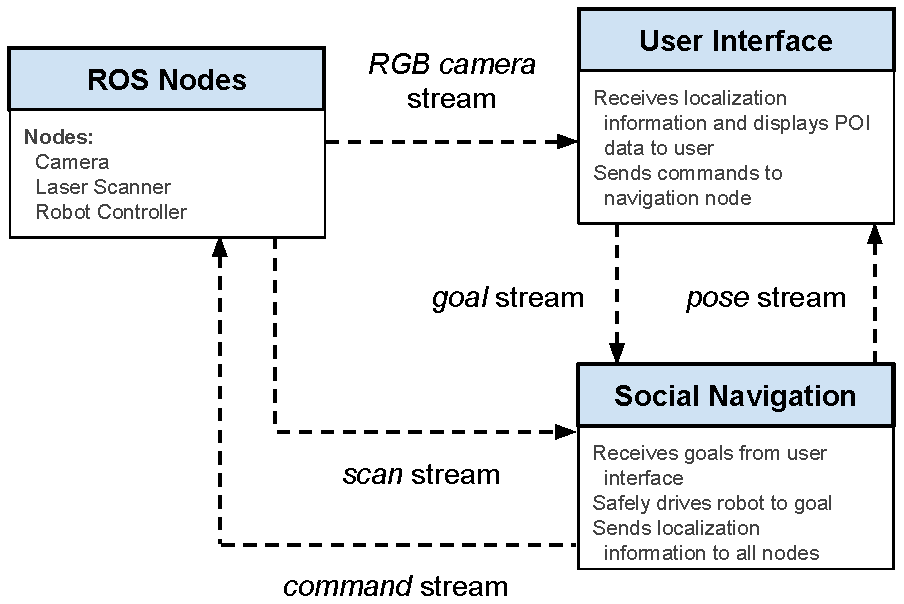
\includegraphics[width=0.75\textwidth]{system_class_overview.pdf}
  \caption{The system architecture showing relationship between high level nodes in the system. The “ROS Nodes” are open source nodes (not developed in this project) which provide data to the system and control the robot hardware.}
\end{figure}

Figure \ref{figure:social_navigation} shows the interconnect between Roslyn's internal nodes.
\begin{figure}[t]
 \centering
 \label{figure:social_navigation}
 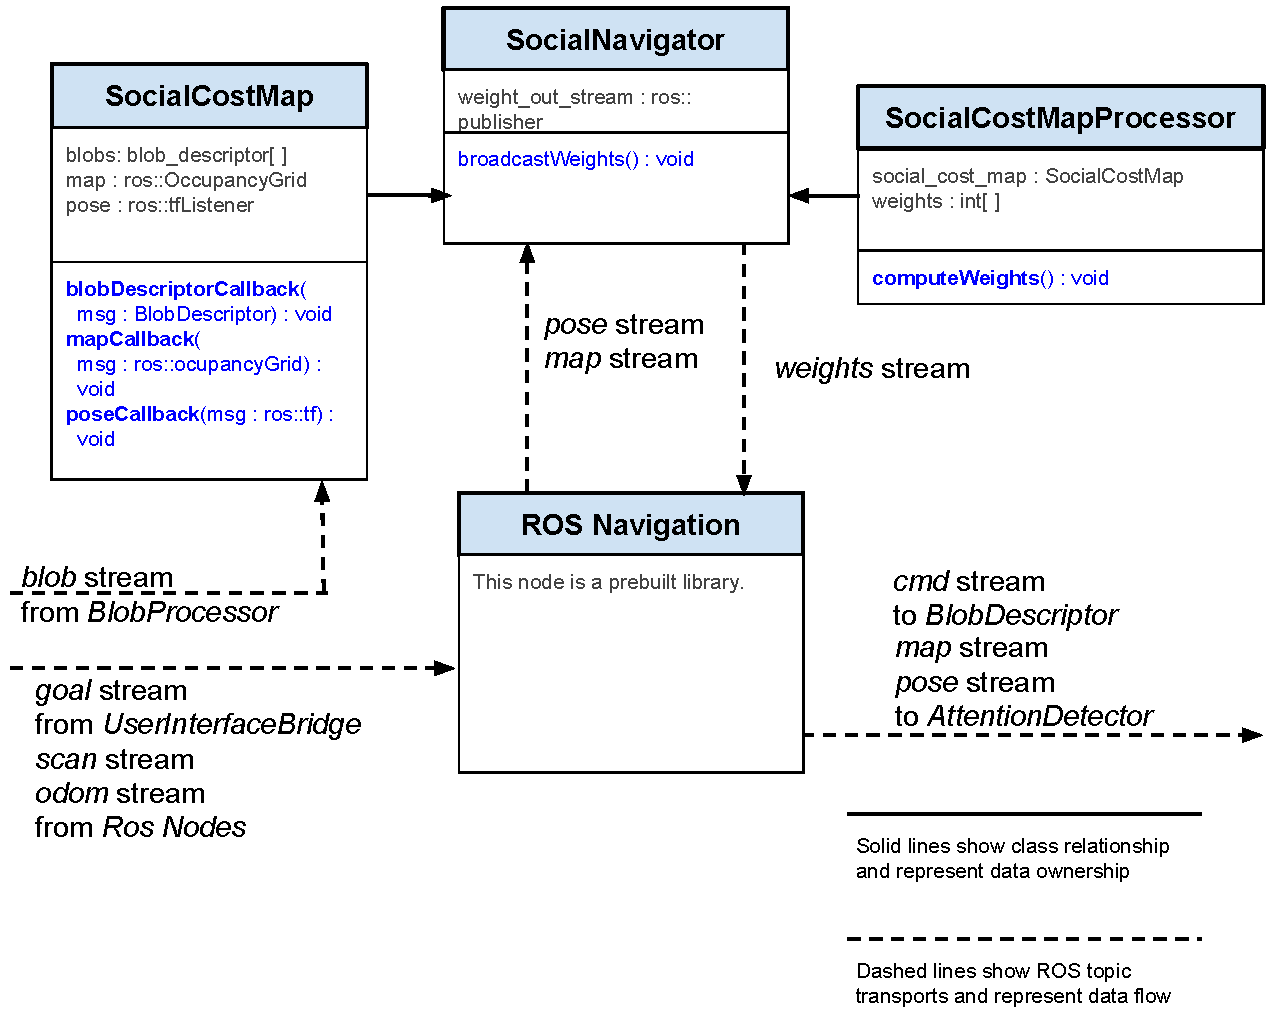
\includegraphics[width=0.75\textwidth]{social_navigation.pdf}
  \caption{Social Navigation class diagram showing the relationship between classes and the rest of the system’s data flow.}
\end{figure}

Figure \ref{figure:social_navigation} shows the internal description of the social navigation components, its intraconnections to itself, and connections to other nodes.
\begin{figure}[t]
 \centering
 \label{figure:social_navigation}
 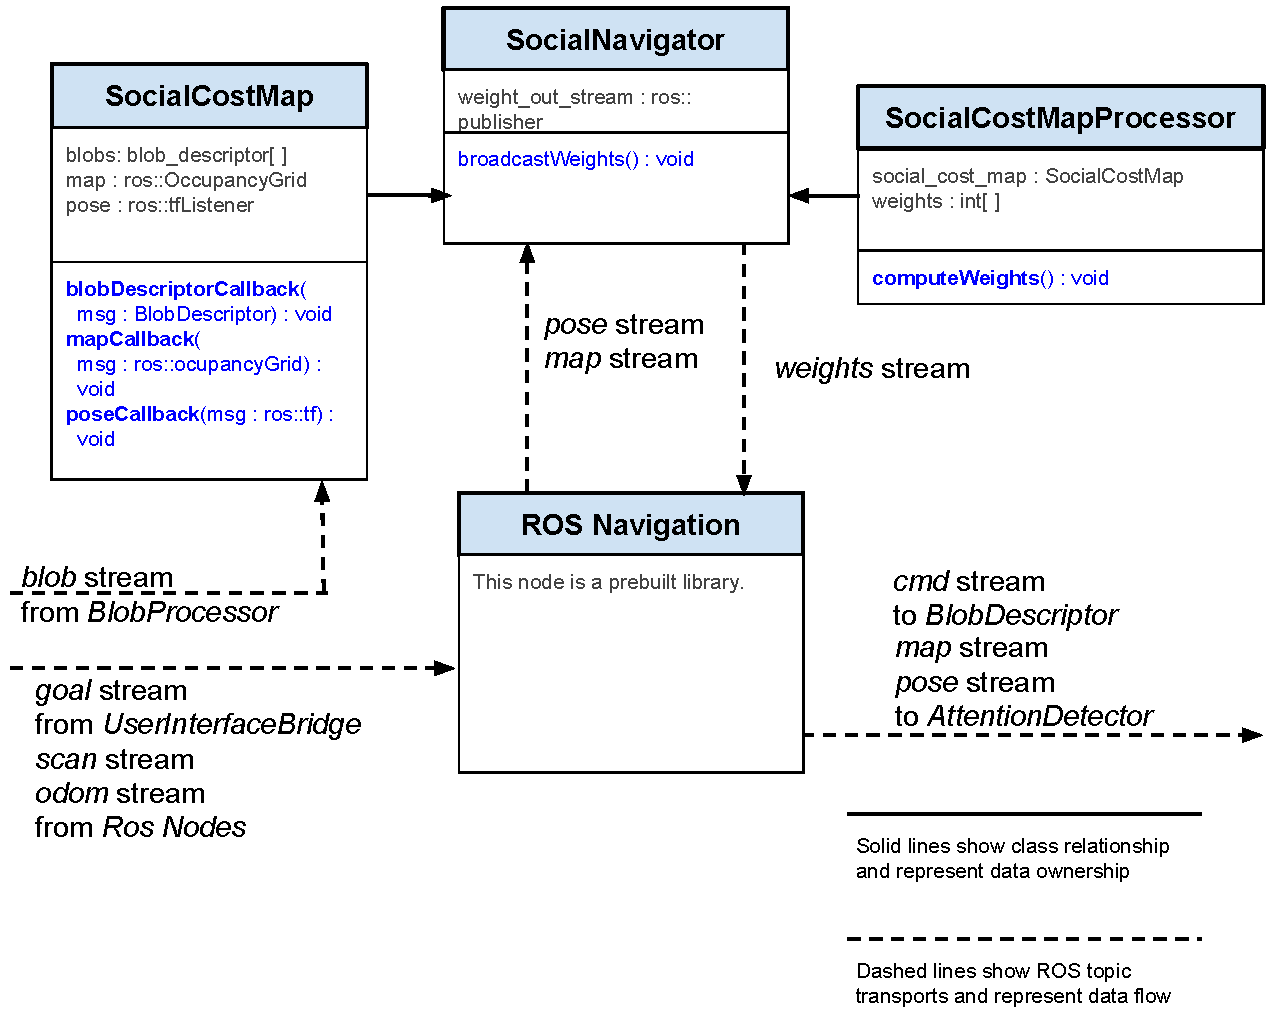
\includegraphics[width=0.75\textwidth]{social_navigation.pdf}
  \caption{Social Navigation class diagram showing the relationship between classes and the rest of the system’s data flow.}
\end{figure}

Figure \ref{figure:user_interface} shows the internal description of the user interface bridge, its intraconnections to itself, and connections to other nodes and to the interface itself.
\begin{figure}[t]
 \centering
 \label{figure:user_interface}
 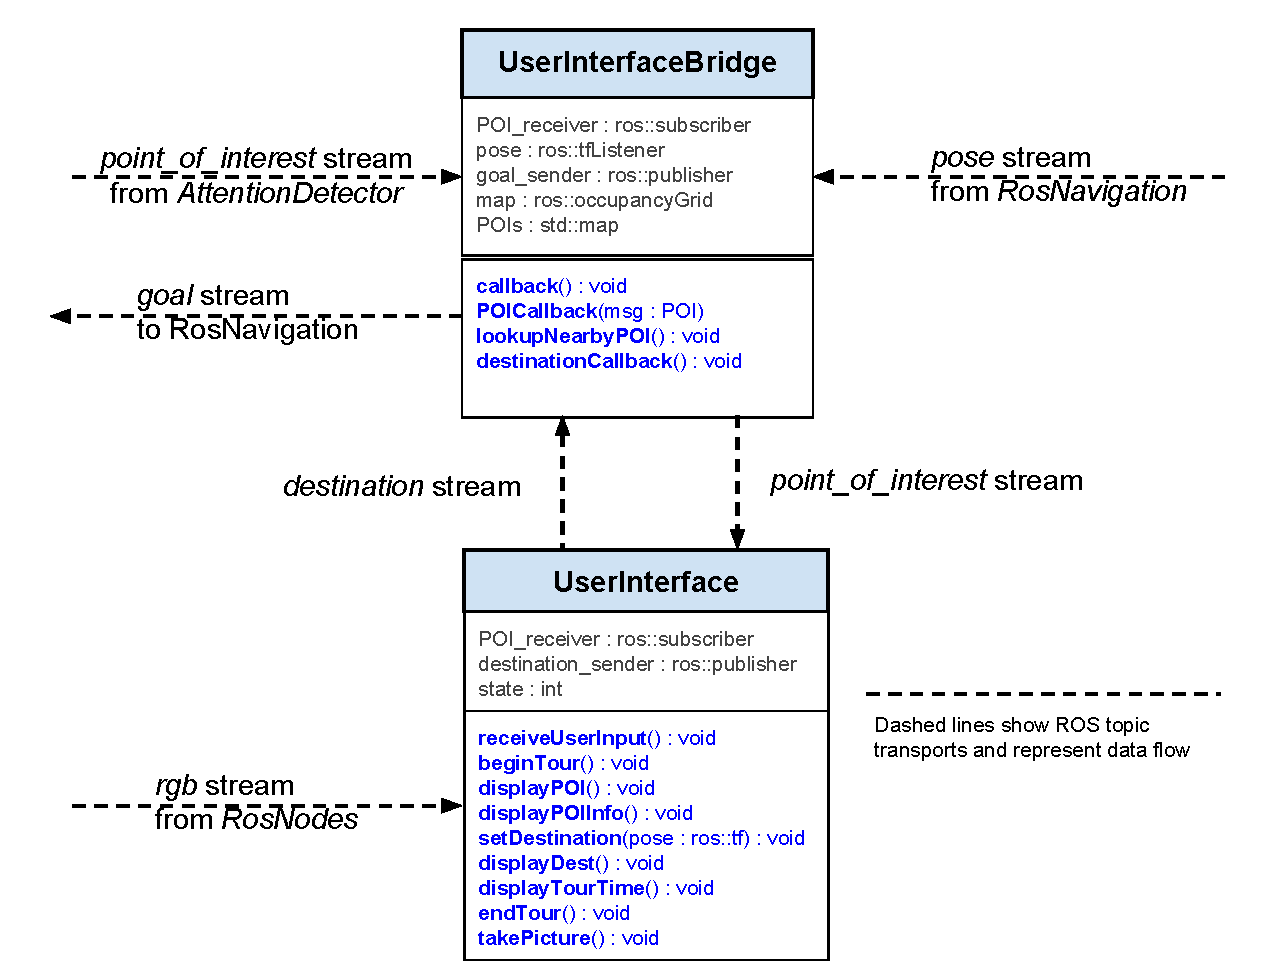
\includegraphics[width=0.75\textwidth]{user_interface.pdf}
  \caption{User Interface class diagram showing the relationship between classes and the rest of the system’s data flow.}
\end{figure}
\subsection{Top Level Activity Diagram}


\bibliographystyle{plain}

\begin{thebibliography}{99}

 \bibitem{USCthesis} \verb=USCthesis2000.sty=,

 \LaTeX\,2\raisebox{-0.2ex}{$\varepsilon$} style file for USC dissertations

 and theses according to the regulations published by the Graduate

 School, Feb 2000.

\end{thebibliography}



\end{document}
